% ==================================================
% Serial Training
% Author: Lester James V. Miranda
% ==================================================

\documentclass[preview, convert={outfile=\jobname.png,density=300}]{standalone}

\usepackage{tikz}
\usepackage{color}
\usepackage{subfig}
\usepackage{ifthen}

\renewcommand\familydefault{\sfdefault}

\usetikzlibrary{
    matrix,
    shapes,
    fit,
    arrows.meta,
    arrows,
    positioning,
    calc,
    backgrounds,
    shadows.blur,
    shapes.geometric,
}

\begin{document}
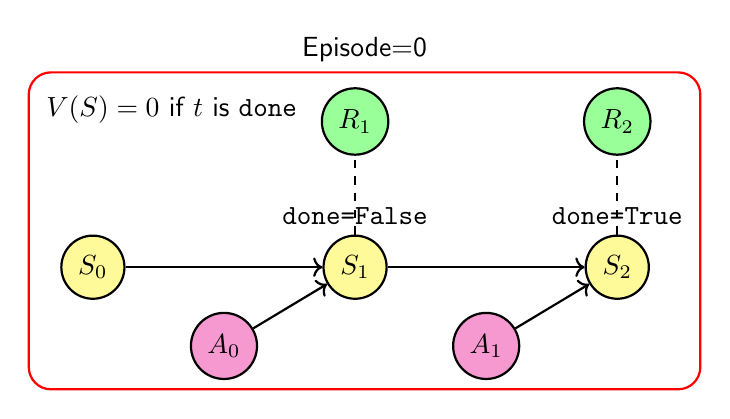
\begin{tikzpicture}[
    node distance= 1cm and 2.5cm,
    proc/.style={draw, circle, thick, minimum size=0.75cm},
    state/.style={proc, fill=yellow!40},
    action/.style={proc, fill=magenta!40},
    reward/.style={proc, fill=green!40},
    episode/.style={draw, color=red, fill=none, rounded corners=8pt,thick, inner xsep=1mm},
    textbox/.style={fill=white, align=center, minimum height=0.7cm, minimum width=0.7cm},
]

\node[state] (s0) at (0,0) {$S_0$};
\node[state] (s1) [right=of s0, label={\texttt{done=False}}] {$S_1$};
\node[state] (s2) [right=of s1, label={[name=terminus]\texttt{done=True}}] {$S_2$};

\node[action] (a0) at ([yshift=-1cm]$(s0)!0.5!(s1)$) {$A_0$};
\node[action] (a1) at ([yshift=-1cm]$(s1)!0.5!(s2)$) {$A_1$};

\node[reward] (r1) [above=of s1] {$R_1$};
\node[reward] (r2) [above=of s2] {$R_2$};

\draw[->, thick] (s0) -- (s1) {};
\draw[->, thick] (s1) -- (s2) {};
\draw[->, thick] (a0) -- (s1) {};
\draw[->, thick] (a1) -- (s2) {};
\draw[dashed, thick] (s1) -- (r1) {};
\draw[dashed, thick] (s2) -- (r2) {};

\node[textbox] (textbox) at (1,2) {$V(S)=0$ if $t$ is \texttt{done}};

\begin{scope}[on background layer]
    \node [episode, fit=(textbox)(s0)(r2)(a1)(terminus), label={Episode=0}] {};
\end{scope}


\end{tikzpicture}
\end{document}
